\documentclass[12pt,a4paper]{article}
\usepackage[utf8]{inputenc}
\usepackage[spanish]{babel}
\usepackage{graphicx}
\usepackage{kpfonts}
\usepackage[left=2cm,right=2cm,top=2cm,bottom=2cm]{geometry}
\begin{document}
\title{Universidad politecnica\\ de la \\ Zona Metropolitana\\ de Guadalajara}
\author{Tarea 6\\ Angel Eraclio Briano Garcia 18311625\\ Ing. Mecatronica 4B}
\maketitle
\begin{figure}[h!]
\centering

\includegraphics[scale=1]{untitled.png} 
\end{figure}
\newpage
 

\section{Diseño de modulacion de ancho de pulso (PWM) con Amp-Op y transistotes}
Los conversores DC/AC
tienen por objetivo la transformación de tensión DC a
tensión AC de amplitud y/o
frecuencia variable dependiendo de la aplicación. El
proceso de conversión de
voltaje se logra mediante la
implementación de técnicas
de modulación, las cuales actúan sobre un puente inversor monofásico o trifásico.
Según las características de
estas técnicas, las propiedades de eficiencia en la conversión, contenido armónico
de la señal de salida y pérdidas en el puente inversor
cambian. En el presente
artículo se da un repaso de diferentes técnicas de modulación escalares (PWM) y vectoriales (SVM), enfatizando
en las vectoriales por ser las
más utilizadas actualmente
en los sistemas drive para
motores de inducción y en sistemas de alimentación trifásica, a la vez que presenta
las mejores características de
desempeño que las técnicas
de modulación escalares o
PWM (Modulación por Ancho de Pulso).
\begin{figure}[h!]
\centering
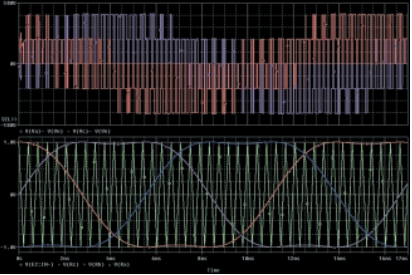
\includegraphics[scale=1]{Captura.PNG} 
\end{figure}
\subsection{Introduccion}
Los circuitos de conversión DC/
AC tienen amplia aplicación en la
industria. Son utilizados en variadores de velocidad, sistemas de alimentación ininterrumpida, filtros
activos, etc. Los conversores DC/
AC se clasifican como inversores
con fuente de voltaje (VSI) e inversores con fuente de corriente
(CSI).1,2 Los CSI se usan en sistemas de alta potencia, los VSI se reservan para aplicaciones en baja y
mediana potencia. Dentro de esta
clasificación existen varias configuraciones de conversores DC/AC que
dependen de la aplicación final y el
nivel de voltaje o corriente de su
salida. En el caso de los drive para
motores de baja y mediana potencia, la topología típica es el medio
puente inversor trifásico con fuente
de voltaje (Figura 1), formado por
seis elementos de conmutación
Mosfet’s, Transistores Bipolares de
Compuerta Aislada (IGBT), Tiristores desactivados por Compuerta
(GTO) o Tiristores Controlados por
MOS (MCT.
Adicionalmente, se debe considerar la técnica de modulación que activará los elementos de conmutación.
En el inversor con fuente de voltaje
la técnica de modulación se encarga
de la forma de onda de la señal de
salida AC, su nivel de tensión y su frecuencia. Las técnicas de modulación se pueden clasificar en escalares
o PWM («Pulse Width Modulation»),6,9 y vectorialeso SVM («Space Vector Modulation»).10,13 Entre las
técnicas escalares se encuentran la
técnica de modulación de onda cuadrada (six-step), técnica de modulación sinusoidal, técnica de modulación sinusoidal con tercer armónico,
entre otras; divisibles a la vez en técnicas de modulación basadas en portadora triangular (carrier based) y técnicas programadas.7
 La técnica de
modulación SVM se presenta en los
años ochentas la cual maneja el puente inversor trifásico como una unidad
y se basa en la representación vectorial del voltaje trifásico para el manejo del puente inversor, disminuye las
pérdidas por conmutación en el mismo y minimiza el contenido armónico de la señal de salida.
\begin{figure}[h!]
\centering
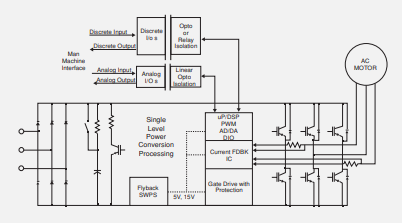
\includegraphics[scale=1]{Captura1.PNG} 
\end{figure}
\subsection{Técnicas de modulación
escalares o PWM}
Se usa en inversores DC/AC
monofásicos y trifásicos. Se basan
en la comparación de una señal de
referencia a modular y una señal
portadora de forma triangular o
diente de sierra (Figura 2); la comparación generará un tren de pulsos
de ancho específico que se utilizan
en la conmutación del puente inversor. La relación entre la amplitud de
la señal portadora y la señal de referencia se llama «índice de modulación» y se representa por «ma»
(1), donde Ar es la amplitud de la
señal de referencia y Ac es la amplitud de la señal portadora. El índice de modulación permite obtener tensión variable a la salida del
inversor.
\begin{figure}[h!]
\centering
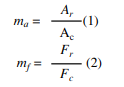
\includegraphics[scale=1]{Captura2.PNG} 
\end{figure}
La relación entre la frecuencia de
la señal portadora y la frecuencia de
referencia se denomina «índice de
frecuencia» y se representa por «mf»
(2), idealmente mf debe ser mayor a
21 y la frecuencia de la portadora
múltiplo de la frecuencia de la señal
de referencia.15 El índice de frecuencia determina la distorsión armónica de la señal de salida la cual es una
medida de su contenido armónico.
La variación de la señal de referencia y la secuencia de conmutación
dan como resultado diferentes técnicas de modulación PWM, cada una
modifica la eficiencia de la conversión, las pérdidas por conmutación
en el puente inversor y la pureza de
la señal de salida.
\begin{figure}[h!]
\centering
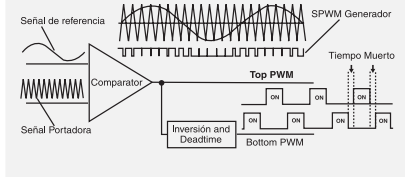
\includegraphics[scale=1]{Captura3.PNG} 
\end{figure}
\newpage
\subsection{Modulacion PWM a 60°}
la técnica de modulación PWM a
60° se basa en la adición de ZSS.
El objetivo es «achatar» la forma de
onda de voltaje de salida desde los
60° hasta los 120° y desde 240° a
300°. Los dispositivos del puente
inversor se mantienen encendidos
durante un tercio de ciclo, se presentan menos pérdidas por conmutación. La técnica de modulación
PWM a 60° aprovecha mejor la tensión del bus de DC, alcanzando una
tensión de fase igual a 0.57735Vdc
\begin{figure}[h!]
\centering
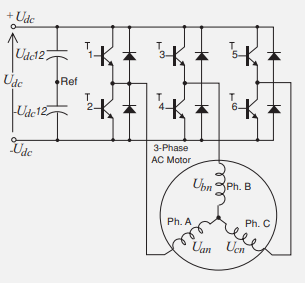
\includegraphics[scale=1]{Captura4.PNG} 
\end{figure}
\section{Bibliografia}
Posada Contreras, Johnny
Modulación por ancho de pulso (PWM) y modulación vectorial (SVM). Una introducción a las técnicas
de modulación
El Hombre y la Máquina, núm. 25, julio-diciembre, 2005, pp. 70-83
Universidad Autónoma de Occidente
Cali, Colombia
\end{document}